%==============================================================================
%  SuperMoTo — User & Technical Manual
%
%  Build:  pdflatex SuperMoTo.tex   (run twice for the table of contents /
%          cross-references). Requires TikZ; no external images are mandatory
%          to compile — every screenshot is a placeholder with a written
%          description so the document builds before the screenshots exist.
%
%  (c) 2023-2026 Olivier Doaré — LGPL-3.0-or-later
%==============================================================================
\documentclass[11pt,a4paper]{report}

\usepackage[utf8]{inputenc}
\usepackage[T1]{fontenc}
\usepackage{lmodern}
\usepackage[margin=2.5cm]{geometry}
\usepackage{graphicx}
\usepackage{xcolor}
\usepackage{tikz}
\usetikzlibrary{positioning,arrows.meta,calc,fit,backgrounds,shapes.geometric}
\usepackage{pgfplots}
\pgfplotsset{compat=1.17}
\usepackage{booktabs}
\usepackage{tabularx}
\usepackage{enumitem}
\usepackage{amsmath}
\usepackage{amssymb}
\usepackage{siunitx}
\usepackage{fancyhdr}
\usepackage[colorlinks=true,linkcolor=smtblue,urlcolor=smtblue,citecolor=smtblue]{hyperref}

%-- Theme colours (loosely follow the plugin Theme.h) -------------------------
\definecolor{smtblue}{HTML}{2E6DB4}
\definecolor{smtgold}{HTML}{C9A227}
\definecolor{smtpanel}{HTML}{2B2F36}
\definecolor{smtlight}{HTML}{EEF1F5}
\definecolor{smtgreen}{HTML}{3FA34D}

%-- A reusable box for the "screenshot goes here" placeholders ----------------
% Usage: \screenshot{label}{caption / description of what to capture}
% Includes figures/#1 when it exists, otherwise draws a framed placeholder with
% the description, so the document builds before every screenshot is captured.
\newcommand{\screenshot}[2]{%
  \begin{figure}[ht]
  \centering
  \IfFileExists{figures/#1}{%
    \includegraphics[width=0.9\textwidth]{figures/#1}%
  }{%
    \fbox{\parbox[c][0.22\textwidth][c]{0.86\textwidth}{\centering
      \itshape [screenshot to capture: \texttt{#1}]\par\medskip
      \normalfont\footnotesize #2}}%
  }%
  \caption{#2}
  \label{fig:#1}
  \end{figure}}

\pagestyle{fancy}
\fancyhf{}
\rhead{\textsc{SuperMoTo}}
\lhead{\leftmark}
\rfoot{\thepage}

\title{{\Huge\textbf{SuperMoTo}}\\[0.4em]
       \textit{The Super Monitoring Tool}\\[0.4em]
       \Large Monitoring Matrix, Measurement \& Speaker Correction\\[1.2em]
       \large User and Technical Manual}
\author{Olivier Doaré, ENSTA
\\ \texttt{https://perso.ensta.fr/{\textasciitilde}doare}
\\ \texttt{github.com/odoare}
\\ FX-Mechanics}
\date{Document version 0.1 — \today}

%==============================================================================
\begin{document}
\maketitle
\tableofcontents

%==============================================================================
\chapter{Overview}
%==============================================================================

\section{What SuperMoTo is}
SuperMoTo is an FX-Mechanics audio plugin (VST3, AU and Standalone) for the
\emph{monitoring section} of a studio. It is the big brother of
\href{https://github.com/odoare/MoTo}{MoTo}. From a single instance it lets you:

\begin{itemize}[nosep]
  \item route up to \textbf{16 inputs to 16 outputs} through a full routing
        matrix, with per-crosspoint gain, EQ, phase and delay;
  \item apply \textbf{one FIR correction filter per output} (zero-latency WDL
        convolution) to flatten each loudspeaker;
  \item \textbf{measure} the loudspeakers in the room with built-in stimuli;
  \item \textbf{analyse} those measurements and \textbf{design} the FIR
        correction curves (magnitude and phase), including phase-coherent
        \textbf{subwoofer integration}.
\end{itemize}

The plugin is organised in three functional parts that share one engine:
the \textbf{Monitoring matrix} (Chapter~\ref{ch:matrix}), the
\textbf{Measurement / Calibration} view (Chapter~\ref{ch:measure}) and the
\textbf{Analysis \& correction design} view (Chapter~\ref{ch:analysis}).

\section{Why calibrate a monitoring system?}\label{sec:why}
What you hear at the listening position is never the loudspeaker alone: it is
the loudspeaker \emph{convolved with the room}, sampled by the microphone (or
your ears) at one place. Several independent mechanisms each leave their mark
on that combined response, and they behave very differently --- which is
exactly why some of them can be corrected electronically and some cannot.

\subsection{The room's low-frequency modes}
Below roughly the \textbf{Schroeder frequency} (typically \SIrange{150}{300}{\hertz}
in a domestic-sized room), the room behaves as a small set of discrete
resonances --- standing waves between parallel surfaces. Each \textbf{room
mode} stores energy and releases it slowly, producing large peaks and dips in
the magnitude response (often \SI{10}{\decibel} or more) together with audible
\textbf{ringing} (slow modal decay) in the time domain. Modes are strongly
position dependent: a dip at one seat can be a peak half a metre away.

\subsection{Boundary and early reflections}
Sound radiated towards nearby surfaces returns to the listener delayed and
attenuated. Reflections off the desk, floor, ceiling and side walls combine
with the direct sound to produce \textbf{comb filtering} (regularly spaced
peaks and notches) across the midrange and treble, and the speaker--boundary
interference (\textbf{SBIR}) cancellation places a characteristic dip in the
upper bass whose frequency is set by the speaker-to-wall distance. Unlike
modes these are essentially \emph{wide-band} and tied to geometry.

\subsection{Imperfect loudspeakers}
Even in an anechoic chamber no speaker is perfectly flat: drivers have their
own magnitude ripple and roll-offs, and the crossover between drivers adds
\textbf{phase} shift, so the speaker is not minimum-phase everywhere. This part
of the error is a property of the box, is the \emph{same} at every listening
position, and is the most cleanly correctable.

\subsection{Subwoofers and the crossover region}
Adding a subwoofer introduces a second source, in a different place, with its
own roll-off and delay. Where the sub and the mains overlap their outputs add
as \emph{complex} pressures: unless they are in phase through the crossover the
sum shows a dip or, worse, a deep cancellation~\cite{Linkwitz1976}. Getting a
smooth, coherent hand-off is as much a \textbf{phase / timing} problem as a
level problem.

\subsection{What SuperMoTo can and cannot do}
Correction is a linear filter applied to the signal \emph{before} the speaker.
That makes it powerful for some of the problems above and powerless for others:

\begin{itemize}[nosep]
  \item \textbf{Can do well.} Flatten the loudspeaker's own magnitude and phase
        response; tame the broad \emph{minimum-phase} part of the
        room's low-frequency response that is common to the listening area;
        apply a defensible target/house curve; and \textbf{time- and
        phase-align a subwoofer} with the mains so they sum coherently through
        the crossover.
  \item \textbf{Cannot do.} It cannot remove energy that arrives \emph{later}
        than the direct sound --- a reflection is a separate event in time, so
        ``correcting'' for it only pre-distorts the direct sound and the dip
        usually returns elsewhere. Deep cancellation notches are
        \emph{non-minimum-phase} and effectively non-invertible: boosting into
        them wastes headroom and excites the mode further rather than filling
        the null~\cite{NeelyAllen,Mourjopoulos1994}. And because the
        measurement is taken around one reference area, a correction is only
        valid \emph{there} --- it cannot be flat everywhere at once~\cite{Toole}.
\end{itemize}

This is why SuperMoTo derives its correction from a \textbf{spatial average} of
several microphone positions (so it follows the response that is consistent
across the listening area rather than chasing one seat's interference notches),
limits its boost with a soft ceiling, and smooths the target more coarsely as
frequency rises (Chapter~\ref{ch:analysis}).

\subsection{Treat the room first}
Electronic correction is the \emph{last} step, not a substitute for acoustics.
The errors it handles worst --- reflections and modal ringing --- are precisely
the ones that respond to physical treatment, so the most effective gains come
\textbf{upstream}, before any filter is designed:

\begin{itemize}[nosep]
  \item \textbf{Placement} of speakers and listening position relative to the
        walls (avoiding strong SBIR dips and the worst modal seats).
  \item \textbf{Symmetry} of the left/right setup, so the stereo image is not
        skewed by the room.
  \item \textbf{Bass trapping} in the corners to shorten modal decay --- this
        reduces ringing, which no magnitude filter can.
  \item \textbf{Broadband absorption} at the first reflection points to reduce
        comb filtering.
\end{itemize}

A well-treated room makes the residual error smoother, more minimum-phase and
more uniform across positions --- exactly the kind of error a filter
\emph{can} fix --- so room treatment and SuperMoTo are complementary, in that
order.

\section{Signal flow at a glance}
Figure~\ref{fig:signalflow} shows the per-block processing performed by the
matrix engine. Audio enters on 16 discrete input channels, is summed through
the active matrix configuration(s), passes the per-output trim and FIR
correction, is time-aligned across outputs, and finally the master section
(Level / Mute / Dim / Mono) is applied before the 16 discrete outputs.

\begin{figure}[ht]
\centering
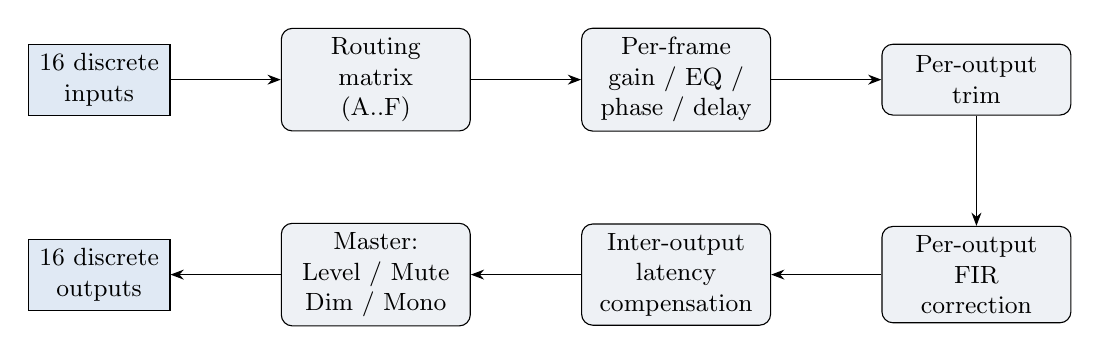
\begin{tikzpicture}[
   node distance=8mm and 14mm,
   block/.style={draw, rounded corners, fill=smtlight, minimum height=9mm,
                 minimum width=24mm, align=center, font=\small},
   io/.style={draw, fill=smtblue!15, minimum height=9mm, minimum width=18mm,
              align=center, font=\small},
   >={Stealth[]}]
  \node[io] (in) {16 discrete\\inputs};
  \node[block, right=of in] (matrix) {Routing\\matrix\\(A..F)};
  \node[block, right=of matrix] (frame) {Per-frame\\gain / EQ /\\phase / delay};
  \node[block, right=of frame] (trim) {Per-output\\trim};
  \node[block, below=14mm of trim] (fir) {Per-output\\FIR\\correction};
  \node[block, left=of fir] (comp) {Inter-output\\latency\\compensation};
  \node[block, left=of comp] (master) {Master:\\Level / Mute\\Dim / Mono};
  \node[io, left=of master] (out) {16 discrete\\outputs};

  \draw[->] (in) -- (matrix);
  \draw[->] (matrix) -- (frame);
  \draw[->] (frame) -- (trim);
  \draw[->] (trim) -- (fir);
  \draw[->] (fir) -- (comp);
  \draw[->] (comp) -- (master);
  \draw[->] (master) -- (out);
\end{tikzpicture}
\caption{Per-block signal flow of the matrix engine. Each crosspoint
(``frame'') of the matrix has its own gain, 4-band EQ, phase inversion and
fractional delay; each output has a trim and an optional FIR correction
filter. Outputs are then re-aligned so loudspeakers with different FIR
lengths stay time-coherent.}
\label{fig:signalflow}
\end{figure}

\section{Plugin format and channel layout}
\begin{itemize}[nosep]
  \item Formats: \textbf{VST3}, \textbf{AU}, \textbf{Standalone}.
  \item Bus layout: one input bus and one output bus, each
        \textbf{16 discrete channels}
        (\texttt{AudioChannelSet::discreteChannels(16)}). The plugin only
        reports support for the exact 16-in / 16-out layout.
  \item Plugin type: audio effect (not a synth, no MIDI).
\end{itemize}

This fixed 16$\times$16 discrete layout is the key constraint for host
compatibility — see Chapter~\ref{ch:daw}.

%==============================================================================
\chapter{Host (DAW) compatibility}\label{ch:daw}
%==============================================================================

SuperMoTo is primarily designed and tested in \textbf{REAPER}. To host it
usefully a DAW must satisfy two requirements:

\begin{enumerate}[nosep]
  \item \textbf{Flexible channel routing} — the ability to feed the plugin's
        16 discrete inputs from arbitrary sources and to send its 16 discrete
        outputs to arbitrary hardware outputs / busses.
  \item \textbf{A monitoring (control-room) insert point} — a place to put the
        plugin on the path between the mix and the physical speaker outputs,
        \emph{after} the program material is mixed but \emph{before} it leaves
        for the monitors, ideally not printed into renders/bounces.
\end{enumerate}

\section{Recommended and likely-compatible hosts}
\begin{table}[ht]
\centering
\renewcommand{\arraystretch}{1.3}
\begin{tabularx}{\textwidth}{l c X}
\toprule
\textbf{Host} & \textbf{Fit} & \textbf{Notes} \\
\midrule
REAPER & \textbf{Primary} &
  Per-track/track-channel routing up to 64 channels, and a dedicated
  \emph{Monitoring FX} chain (\textsf{View\,$\rightarrow$\,Monitoring FX})
  that sits on the hardware output path and is excluded from renders. The
  reference environment. \\
Ardour & Strong &
  Arbitrary bus channel counts and flexible port routing; a dedicated
  \emph{Monitor Section} on the master/monitor path. A natural fit on Linux. \\
Steinberg Nuendo / Cubase & Strong &
  The \emph{Control Room} provides a monitor insert chain with flexible
  downmix and multi-channel busses — ideal for a post-production monitoring
  matrix. Confirm the Control Room insert accepts a 16-channel plugin layout. \\
Bitwig Studio & Possible &
  Very flexible routing and per-device chains; place the plugin on the master
  or on a hardware-output chain. No formal ``monitor section'', so the
  monitoring insert must be built manually and bypassed before export. \\
Standalone (built in) & Always &
  The Standalone build talks straight to the audio device (16 in / 16 out if
  the interface provides them); useful for a dedicated monitor-controller
  machine with no DAW. \\
\bottomrule
\end{tabularx}
\caption{Hosts that can drive SuperMoTo. ``Fit'' is the author's assessment
based on the routing / monitor-section requirements; only REAPER is formally
tested.}
\label{tab:hosts}
\end{table}

\section{Hosts likely to be awkward}
\begin{itemize}[nosep]
  \item \textbf{Pro Tools} — plugin channel formats are constrained to named
        surround layouts; an arbitrary 16-channel discrete insert is not the
        native model.
  \item \textbf{Logic Pro} — surround formats are fixed and discrete
        16-channel routing through a monitor insert is not straightforward.
  \item \textbf{Studio One / FL Studio / Live} — usable as generic effect
        hosts, but they lack a true control-room monitor insert, so the
        plugin would have to live on the master bus and be manually bypassed
        for exports.
\end{itemize}

\section{Suggested REAPER setup (reference)}
\begin{enumerate}[nosep]
  \item Open \textsf{View\,$\rightarrow$\,Monitoring FX} and insert SuperMoTo
        there so it processes the hardware output path and is excluded from
        renders.
  \item In the plugin's pin connector / channel mapping, map your mix busses
        to inputs 1..N and the plugin outputs 1..M to the physical speaker
        outputs.
  \item Build your routing in the matrix (or with the Configuration tool) and
        store rigs in configurations A..F.
\end{enumerate}

% TODO(screenshot): REAPER Monitoring FX window with SuperMoTo inserted and
% the 16x16 pin connector visible.
\screenshot{reaper-monitoring-fx.png}{REAPER ``Monitoring FX'' window with
SuperMoTo inserted, showing the 16-in/16-out pin/channel mapping to the
hardware outputs.}

%==============================================================================
\chapter{The monitoring matrix}\label{ch:matrix}
%==============================================================================

% TODO(screenshot): full plugin window in Matrix view: top bar (A..F, Exclusive,
% Level, Mute/Dim/Mono, collapse), the 16x16 grid of frames with vu-meters,
% the output strip along one edge, the analyzer, and the frame editor panel.
\screenshot{SuperMoTo_matrix_view.png}{The Matrix view: top bar with configuration
buttons A--F, Exclusive toggle, master Level and Mute/Dim/Mono; the 16$\times$16
grid of frames each with its vu-meter; the per-output strip; the global
spectrum analyzer; and the frame editor panel (bottom-right).}

\section{Concepts}
The matrix is a \textbf{16$\times$16 grid}. The cell at row \emph{in},
column \emph{out} is a \textbf{frame} (crosspoint): it controls how much of
input \emph{in} is sent to output \emph{out} and how it is processed on the
way. Each output also has global \textbf{output settings} (trim + FIR) that
describe the physical loudspeaker attached to it and are therefore shared by
all configurations.

\subsection{What a frame contains}
\begin{itemize}[nosep]
  \item \textbf{Active} flag (is this crosspoint routed at all);
  \item \textbf{Gain} (overall frame level, dB);
  \item a \textbf{4-band EQ} — each band can be lowpass, highpass, bandpass
        or peaking; lowpass/highpass are 2nd or 4th order; bands are cascaded
        in series;
  \item \textbf{Phase invert};
  \item \textbf{Delay}, \SI{0}{\milli\second} to \SI{100}{\milli\second},
        fractional (sub-sample);
  \item a \textbf{vu-meter} and an \textbf{analyzer} checkbox to show the
        frame's signal on the spectrum analyzer.
\end{itemize}

\begin{figure}[ht]
\centering
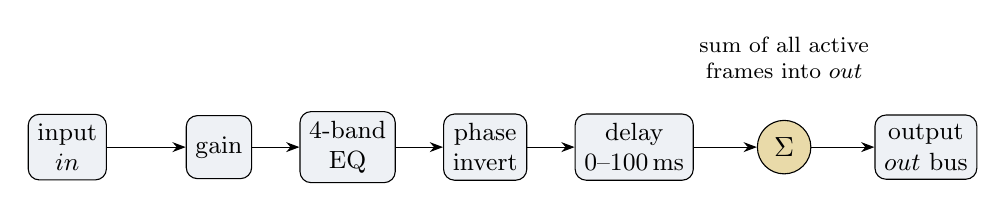
\begin{tikzpicture}[
   block/.style={draw, rounded corners, fill=smtlight, minimum height=8mm,
                 align=center, font=\small},
   >={Stealth[]}, node distance=6mm]
  \node[block] (in) {input\\$in$};
  \node[block, right=10mm of in] (gain) {gain};
  \node[block, right=6mm of gain] (eq) {4-band\\EQ};
  \node[block, right=6mm of eq] (phase) {phase\\invert};
  \node[block, right=6mm of phase] (delay) {delay\\0--100\,ms};
  \node[draw, circle, right=8mm of delay, fill=smtgold!40] (sum) {$\Sigma$};
  \node[block, right=8mm of sum] (out) {output\\$out$ bus};
  \draw[->] (in) -- (gain);
  \draw[->] (gain) -- (eq);
  \draw[->] (eq) -- (phase);
  \draw[->] (phase) -- (delay);
  \draw[->] (delay) -- (sum);
  \draw[->] (sum) -- (out);
  \node[font=\footnotesize, above=4mm of sum, align=center]
    {sum of all active\\frames into $out$};
\end{tikzpicture}
\caption{Processing inside a single frame (crosspoint). Every active frame
feeding a given output is summed into that output's bus before the output
trim and FIR.}
\label{fig:frame}
\end{figure}

\subsection{Configurations A--F}
There are \textbf{6 configurations} (A..F), each a complete 16$\times$16
matrix, stored per preset. They are engaged from the top-bar buttons:
\begin{itemize}[nosep]
  \item \textbf{Exclusive} mode (default): engaging one releases the others —
        an instant A/B between rigs.
  \item \textbf{Non-exclusive} mode: active configurations are \emph{summed},
        so you can stack layers.
\end{itemize}
The configuration you are \emph{editing} is chosen with the ``Edit: A..F''
buttons above the analyzer, independently of which one is engaged for
listening.

\section{Interacting with the matrix}
\begin{table}[ht]
\centering
\renewcommand{\arraystretch}{1.25}
\begin{tabularx}{\textwidth}{l X}
\toprule
\textbf{Gesture} & \textbf{Action} \\
\midrule
Click a frame        & Select it (opens it in the frame editor panel). \\
Double-click a frame & Activate / deactivate the crosspoint. \\
Vertical drag        & Adjust the frame gain. \\
Alt+click            & Toggle the frame's analyzer trace. \\
Right-click          & Context menu for the frame. \\
\midrule
Output: double-click & Toggle that output's FIR on/off. \\
Output: vertical drag& Adjust the output trim. \\
Output: alt+click    & Toggle the output-sum analyzer trace. \\
Output: right-click  & Load / clear the impulse-response (FIR) wav file. \\
\bottomrule
\end{tabularx}
\caption{Mouse interactions in the matrix and output strip. Every page also
has an info button \textbf{(i)} summarising its controls and shortcuts.}
\label{tab:gestures}
\end{table}

\section{Per-output FIR correction and latency compensation}
Each output can carry one \textbf{FIR filter} (loaded from a wav impulse
response, convolved with the zero-latency WDL engine) to compensate the
attached loudspeaker. Because correction IRs are rendered with their energy
\emph{centred} (see Chapter~\ref{ch:analysis}), an FIR of length $L$ adds
about $L/2$ samples of delay to that output.

SuperMoTo applies \textbf{automatic inter-output latency compensation}: among
the outputs fed by the engaged configuration, the ones with shorter (or no)
FIR are delayed so that \emph{all outputs stay time-aligned with the longest
output FIR}. This is what keeps a subwoofer aligned with a linear-phase-
corrected main. A \textbf{gold LED} on an output cell indicates it received
compensation; hover to read the amount.

% TODO(screenshot): close-up of the output strip showing a gold LED on the
% subwoofer output and the hover tooltip with the compensation amount.
\screenshot{latency-led.png}{Output strip close-up: the gold LED marks an output
that received automatic latency compensation; the tooltip shows how many
samples / milliseconds were added to keep it aligned with the longest FIR.}

\section{The global spectrum analyzer}
The analyzer can display any combination of:
\begin{itemize}[nosep]
  \item individual matrix \textbf{frames} (alt+click / frame checkbox), up to
        8 simultaneous frame traces;
  \item \textbf{output sums} (output-strip checkbox).
\end{itemize}
A clickable \textbf{avg / peak} badge switches the per-point aggregation. The
analyzer also has buttons to change the vertical-axis limits, and zooming is
driven by mouse interaction on the plot.

\section{The Configuration tool}
For standard layouts the Configuration tool writes a whole matrix for you.
Choose a layout (\textbf{2.0, 2.1, 4.0, 5.1, 7.1}), assign the input and
output channel of each speaker, set the gains and the bass-management
crossover frequency, then \textbf{Apply} to a configuration (A..F). The mains
are high-passed and their sum is sent, low-passed, to the subwoofer output.
The result is an ordinary configuration you can fine-tune by hand afterwards.

% TODO(screenshot): the Configuration tool dialog with a 5.1 layout selected,
% per-speaker input/output assignment, gains, and the crossover control.
\screenshot{config-tool.png}{The Configuration tool: a standard layout (here 5.1)
with per-speaker input/output assignment, gains and the bass-management
crossover frequency, ready to Apply into one of the A--F configurations.}

\section{Host-automatable parameters}
The matrix settings themselves are deliberately \emph{not} exposed as host
parameters: $6 \times 16 \times 16$ frames with $\sim$10 fields each would
swamp any host. They are saved with the plugin state. Only the master
controls are real host parameters:

\begin{table}[ht]
\centering
\renewcommand{\arraystretch}{1.25}
\begin{tabularx}{\textwidth}{l l X}
\toprule
\textbf{Parameter} & \textbf{Type / range} & \textbf{Meaning} \\
\midrule
\texttt{Level}     & float, \SI{-60}{} to \SI{+6}{\dB} & Master output level. \\
\texttt{A}\,\dots\,\texttt{F} & bool (6) & Engage configuration A--F (default: A on). \\
\texttt{Exclusive} & bool (default on) & Engaging one config releases the others; off = sum. \\
\texttt{Mute}      & bool & Mute master output. \\
\texttt{Dim}       & bool & Dim master by \SI{6}{\dB} (factor 0.5). \\
\texttt{Mono}      & bool & Mono sum. \\
\bottomrule
\end{tabularx}
\caption{The complete set of host-automatable parameters (APVTS).}
\label{tab:params}
\end{table}

\section{Compact (collapsed) view}
The collapse button (\textbf{$\blacktriangle$}) shrinks the window to a
compact \emph{output-strip-only} view, handy as a permanent monitor
controller once the routing is set.

%==============================================================================
\chapter{Measurement (Calibration view)}\label{ch:measure}
%==============================================================================

% TODO(screenshot): the Calibration view: microphone input selector, measurement
% type, channel selection, stimulus type, duration/level/base-path controls, the
% Run button, and the SPL meter section on the right with its dual dBFS/dB SPL bar.
\screenshot{calibration-view.png}{The Calibration view: microphone input,
measurement type, channel selection, stimulus (noise / sweep), duration,
level and base path, the Run control, and the right-hand SPL-meter section
with its dual dBFS / dB\,SPL bar and test-signal generators.}

\section{Running a measurement}
Select the \textbf{microphone input}, the \textbf{measurement type}, the
\textbf{channels} to measure, the \textbf{stimulus} (band-limited white noise
or a logarithmic sweep, \SIrange{10}{20000}{\hertz}), the \textbf{duration}
(\SIrange{5}{30}{\second}), the \textbf{level} and the \textbf{base
pathname}. \textbf{Run} measures each selected channel in turn and writes a
stereo wav file per channel:
\begin{itemize}[nosep]
  \item channel 1 = the \textbf{sent} signal (the raw stimulus),
  \item channel 2 = the \textbf{recorded} microphone signal.
\end{itemize}

\section{The measurement microphone}\label{sec:micchoice}
What the analysis sees is the loudspeaker and room \emph{as sampled by the
microphone}. The microphone is therefore part of the measurement chain, and the
kind of microphone — and how well it is characterised — sets a ceiling on how
trustworthy the resulting correction can be.

\subsection{Why a measurement microphone}
Ordinary recording microphones (cardioid vocal or instrument mics) are
deliberately \emph{voiced}: they have a directional pickup pattern and a
shaped, non-flat response designed to flatter sources. That is exactly wrong
for measurement, where you want the microphone to report the sound field as
neutrally as possible. A \textbf{measurement microphone} is built for this:

\begin{itemize}[nosep]
  \item \textbf{Omnidirectional}, so it captures the room as the ear does
        rather than rejecting it from the sides.
  \item \textbf{Small diaphragm} (typically \SI{6}{\milli\metre},
        quarter-inch or half-inch), for a wide, uniform high-frequency
        response with little directional colouration.
  \item \textbf{Nominally flat} magnitude response over the audio band, with
        only small residual deviations — which a calibration file then removes
        (Section~\ref{sec:miccal}).
\end{itemize}

Common, affordable choices include the USB miniDSP \textbf{UMIK-1} / UMIK-2,
the Dayton Audio \textbf{EMM-6} (XLR) and \textbf{iMM-6}, the Behringer
\textbf{ECM8000}, and any class~1/class~2 measurement capsule. USB models carry
their own ADC and appear as a soundcard input; XLR models need phantom power
and an audio interface. Either works — SuperMoTo only needs the microphone to
arrive on one of its plugin input channels.

\subsection{Orientation matters}
Because the microphone is omnidirectional only at low frequencies, its
high-frequency response depends on the angle of arrival, so it is characterised
for a specific \textbf{orientation}:

\begin{itemize}[nosep]
  \item \textbf{\ang{0} (on-axis)} — capsule pointed \emph{at the
        loudspeaker}. This is the orientation for the swept-speaker
        measurements SuperMoTo makes, and the one whose calibration file you
        should load.
  \item \textbf{\ang{90} (grazing)} — capsule pointed at the ceiling,
        used for steady-state room / RTA averaging where sound arrives from
        many directions.
\end{itemize}

Vendors such as miniDSP ship \emph{two} calibration files for this reason; use
the \ang{0} file and point the microphone at the speaker under test.

\section{Microphone calibration}\label{sec:miccal}
% TODO(screenshot): the "Mic cal" control on the first row of the Calibration
% view — the file-name field, the load (...) and clear (x) buttons, next to the
% Microphone input selector.
\screenshot{mic-cal-control.png}{The \textbf{Mic cal} control on the Calibration
view: the loaded file name, the load (\ldots) and clear ($\times$) buttons,
beside the microphone-input selector. The same calibration is shown (read-only)
in the Analysis view.}

\subsection{Why calibrate}
Even a good measurement microphone is not perfectly flat: each capsule has small
deviations from flat, most noticeably a gentle rise or roll-off in the top
octave (above \SIrange{8}{10}{\kilo\hertz}) and sometimes a few tenths of a dB
elsewhere. The \textbf{calibration file} is the measured deviation of that
microphone from flat. If it is not removed, the analysis attributes the
microphone's own colouration to the loudspeaker and \emph{builds it into the
correction} — for example, dipping the speaker's treble to compensate a rise
that exists only in the microphone. Dividing the calibration out first means the
estimated transfer function reflects the \textbf{loudspeaker and room alone}.

\subsection{The calibration file format}
There is no formal standard, but a single de-facto plain-text format is shared
by REW, miniDSP, Dayton (OmniMic / iMM-6) and the FRD tools, and SuperMoTo reads
it directly (\texttt{.txt}, \texttt{.cal} or \texttt{.frd}):

\begin{itemize}[nosep]
  \item comment lines start with \texttt{*}, \texttt{\#} or \texttt{;} (the
        miniDSP \texttt{Sens Factor =\ldots} header is one such line);
  \item every other line is \texttt{frequency\_Hz \quad magnitude\_dB \quad
        [phase\_deg]}, whitespace- or comma-separated, with the phase column
        optional.
\end{itemize}

The magnitude is the microphone's deviation from flat (mean $\approx 0$ in the
midband). Where do the numbers come from? \textbf{Individually-measured} mics
(e.g.\ the UMIK series) have a file keyed to the unit's serial number,
downloaded from the vendor; cheaper mics may ship only a \emph{model-typical}
file, or none. The \texttt{Sens Factor} line encodes absolute sensitivity for
dB\,SPL work and is ignored here — only the frequency-response curve is used.

\subsection{How SuperMoTo applies it}
Because there is only one physical microphone, the calibration is a
\textbf{single global setting}: load it once with \textbf{Mic cal}~\ldots{} on
the Calibration view (it sits next to the microphone-input selector), and it is
remembered across sessions and projects. The Analysis view shows the same
calibration read-only (\textit{Mic cal: \ldots}) as a reminder that it is in
effect. It is used in two places:

\begin{enumerate}[nosep]
  \item \textbf{The live spectrum display} (SPL-meter section) plots the
        \emph{corrected} microphone spectrum, so what you see already has the
        microphone's own response taken out.
  \item \textbf{The analysis} divides the microphone response out of every
        measured transfer function before the average, the correction and the
        exported curves are computed.
\end{enumerate}

Formally, at each frequency bin the measured response is multiplied by the
inverse of the microphone curve,
\begin{equation}
  H_{\text{corr}}(f) = H_{\text{meas}}(f)\;
      10^{-c_{\mathrm{dB}}(f)/20}\; e^{-j\,c_{\phi}(f)},
  \label{eq:miccal}
\end{equation}
where $c_{\mathrm{dB}}$ and $c_{\phi}$ are the calibration magnitude and phase,
interpolated in log-frequency and held flat (at the endpoint value) outside the
file's range. When the file has no phase column, $c_{\phi}\equiv 0$ and only the
magnitude is corrected.

Two consequences are worth stressing:

\begin{itemize}[nosep]
  \item \textbf{The recorded measurement files stay raw.} The calibration is
        applied at \emph{analysis} time, not baked into the captured wavs, so
        you can change or replace the calibration (a better file, the other
        orientation) and simply re-analyse — no need to re-measure.
  \item \textbf{The broadband SPL number is not corrected.} A single dB\,SPL
        reading cannot carry a frequency-dependent curve; only the spectrum
        display and the analysis use the calibration. (Absolute dB\,SPL is set
        separately, Section~\ref{ch:measure}.)
\end{itemize}

\subsection{Practical recommendations}
\begin{itemize}[nosep]
  \item Load the \textbf{\ang{0}} calibration file and point the
        microphone \emph{at the speaker} for the swept measurements.
  \item A calibration matters most \textbf{above a few kHz}, where the
        microphone's own deviations live and where room averaging no longer
        hides them; in the bass the capsule is essentially flat and room modes
        dominate regardless.
  \item Loading \emph{no} calibration is acceptable for broad bass correction,
        but then any treble target inherits the microphone's error — so for
        full-range correction a calibrated microphone is strongly advised.
  \item The calibration corrects the microphone, \emph{not} its placement: mic
        position and spatial averaging (Section~\ref{sec:spatialavg}) remain
        just as important.
\end{itemize}

\section{The three measurement modes}
The \textbf{measurement type} selector decides \emph{where} the stimulus is
injected and \emph{how much} of the engine it passes through before reaching
the loudspeaker and the microphone. The three modes form a natural progression:
characterise a bare speaker (\textbf{Dry}), verify its correction
(\textbf{FIR}), then validate the whole monitored chain (\textbf{System}).
Table~\ref{tab:measmodes} summarises them and Figure~\ref{fig:measmodes} shows
the injection point of each.

\begin{table}[ht]
\centering
\renewcommand{\arraystretch}{1.3}
\begin{tabularx}{\textwidth}{l X l}
\toprule
\textbf{Mode} & \textbf{What is exercised} & \textbf{File name} \\
\midrule
\textbf{Dry} &
  Stimulus written straight onto the measured \emph{output} — no trim, no FIR.
  The raw loudspeaker, as wired. The first step before designing a FIR. &
  \texttt{<base>\_<output>.wav} \\
\textbf{FIR} &
  Stimulus to the measured \emph{output} through its trim and FIR chain only,
  to verify a correction by re-measuring. &
  \texttt{<base>\_<output>.wav} \\
\textbf{System} &
  Stimulus injected into a plugin \emph{input} and run through the whole engine
  (matrix routing, frame EQ / crossover, output FIRs, inter-output latency
  compensation) — the complete system as heard. Channel selection means
  \emph{inputs} in this mode. &
  \texttt{<base>\_in<input>.wav} \\
\bottomrule
\end{tabularx}
\caption{Measurement modes. ``Dry'' characterises a bare speaker, ``FIR''
verifies its correction, ``System'' captures the complete monitored chain.}
\label{tab:measmodes}
\end{table}

\begin{figure}[ht]
\centering
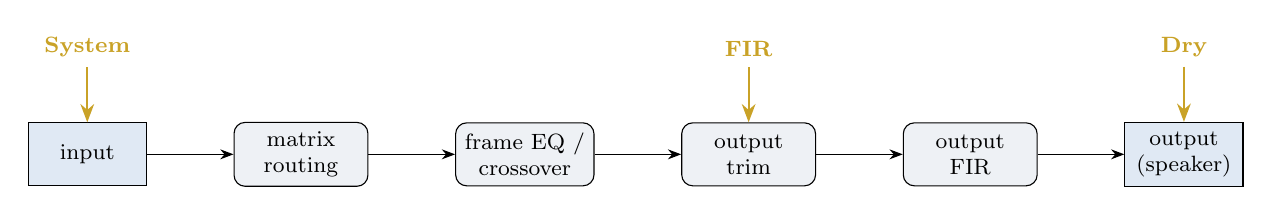
\begin{tikzpicture}[
   node distance=5mm and 11mm,
   block/.style={draw, rounded corners, fill=smtlight, minimum height=8mm,
                 minimum width=17mm, align=center, font=\footnotesize},
   io/.style={draw, fill=smtblue!15, minimum height=8mm, minimum width=15mm,
              align=center, font=\footnotesize},
   inj/.style={smtgold, font=\footnotesize\bfseries},
   >={Stealth[]}]
  \node[io] (in) {input};
  \node[block, right=of in] (matrix) {matrix\\routing};
  \node[block, right=of matrix] (eq) {frame EQ /\\crossover};
  \node[block, right=of eq] (trim) {output\\trim};
  \node[block, right=of trim] (fir) {output\\FIR};
  \node[io, right=of fir] (out) {output\\(speaker)};
  \draw[->] (in) -- (matrix);
  \draw[->] (matrix) -- (eq);
  \draw[->] (eq) -- (trim);
  \draw[->] (trim) -- (fir);
  \draw[->] (fir) -- (out);
  % Injection points
  \draw[->, smtgold, thick] ($(out.north)+(0,7mm)$) node[inj, above]{Dry} -- (out.north);
  \draw[->, smtgold, thick] ($(trim.north)+(0,7mm)$) node[inj, above]{FIR} -- (trim.north);
  \draw[->, smtgold, thick] ($(in.north)+(0,7mm)$) node[inj, above]{System} -- (in.north);
\end{tikzpicture}
\caption{Where each mode injects the stimulus. \textbf{Dry} drives the output
directly (bypassing trim and FIR); \textbf{FIR} enters at the output trim so
the signal passes trim + FIR; \textbf{System} enters at a plugin input and
traverses the entire engine.}
\label{fig:measmodes}
\end{figure}

\subsection{Dry — the raw loudspeaker}
The stimulus is written directly onto the selected output channel; the output
trim and FIR are \emph{not} applied. The capture therefore characterises the
loudspeaker and room exactly as the speaker is physically driven, with no
correction in the path. This is the measurement you feed to the analysis part
(Chapter~\ref{ch:analysis}) to \emph{design} a correction. Run it for each
output you intend to correct, at several microphone positions around the
listening spot.

\subsection{FIR — verifying the correction}
The stimulus is emitted to the selected output through that output's
\textbf{trim and FIR} only (the matrix is otherwise silent). Use it
\emph{after} you have exported a correction IR and assigned it to the output:
re-measuring should show a flatter response than the corresponding Dry
capture. It is the direct before/after check on a single speaker's correction.

\subsection{System — the complete monitored chain}
The stimulus is injected into the selected plugin \emph{input} and run through
the whole engine with the currently engaged configuration(s): matrix routing,
frame EQ and bass-management crossover, the output FIRs and the inter-output
latency compensation — exactly what you hear. The master gain is bypassed
(unity) during the run, so the capture level is set by the stimulus alone.
Because the source is an input, \textbf{the channel selection chooses inputs}
and the files are tagged \texttt{\_in} so a System set never collides with a
Dry/FIR (output) set. This is the end-to-end validation: for a bass-managed
rig it shows whether mains and subwoofer sum smoothly through the crossover at
the listening position.

\subsection{The ``sent'' channel convention}
In \emph{every} mode the captured stereo file stores the \textbf{raw stimulus}
(pre-everything) on channel~1 and the microphone on channel~2. The transfer
function computed in the analysis part is therefore always
\emph{microphone~/~raw\,stimulus}. The consequence is deliberate and
important:
\begin{itemize}[nosep]
  \item in \textbf{Dry} mode that ratio is the bare speaker + room response;
  \item in \textbf{FIR} and \textbf{System} modes it already \emph{includes}
        the correction (and, for System, the full chain), so a successful
        correction shows up directly as a flatter measured transfer function —
        you do not have to subtract anything by hand.
\end{itemize}

\subsection{Capture timing}
Each capture records the stimulus plus a short decay \textbf{tail}
(\SI{1}{\second}) so the room's late energy is included, and the stimulus is
faded in and out (\SI{20}{\milli\second}) to avoid clicks. When measuring
several channels in one run, the engine holds the monitor path silent while
each finished capture is written to disk, so the speakers are not blasted
between consecutive measurements.

\section{The SPL meter}
The right-hand SPL-meter section reuses the microphone / channel /
measurement-type selections. It shows the microphone RMS on a dual
\textbf{dBFS / dB\,SPL} bar and can emit a sine and/or white-noise test
signal, routed exactly like the selected measurement mode. To calibrate the
dB\,SPL scale: play a tone, read a real SPL meter at the listening position,
and type that value into the plugin.

%==============================================================================
\chapter{Analysis \& correction design}\label{ch:analysis}
%==============================================================================

% TODO(screenshot): the Analysis view: loaded measurement set, the transfer-function
% plot (thin individual curves, thick average, correction, corrected response),
% magnitude and phase; the smoothing, correction-level, boost-ceiling and
% analysis-range controls; the subwoofer-integration controls; the export buttons.
\screenshot{analysis-view.png}{The Analysis view: individual smoothed transfer
functions (thin), their average (thick), the proposed correction and the
corrected response, in magnitude and phase; with the nth-octave smoothing,
correction-level, boost-ceiling and analysis-range controls, the subwoofer
integration section, and the Export buttons.}

\section{Transfer-function estimation (Welch method)}
Load the set of measurement files of \emph{one} speaker, the microphone moved
to several positions around the reference listening point. For each file the
plugin estimates the loudspeaker--room transfer function
$H(f)=Y(f)/X(f)$, where $x$ is the emitted stimulus (channel~1 of the file)
and $y$ the captured microphone signal (channel~2). If a microphone
calibration is loaded, it is divided out of $H$ at this stage
(Section~\ref{sec:miccal}, eq.~\eqref{eq:miccal}), so everything below describes
the loudspeaker and room rather than the microphone.

\subsection{The $H_1$ estimator}
A direct bin-by-bin division $Y/X$ is unusable in a room: it is dominated by
measurement noise wherever $X$ is small, and a single FFT gives an estimate
with $100\,\%$ standard error. SuperMoTo instead uses the classical
\textbf{Welch averaged-periodogram} approach~\cite{Welch1967}: the recording
is cut into overlapping segments, each is windowed and transformed, and the
\emph{auto-} and \emph{cross-spectra} are averaged over the $L$ segments,
\begin{equation}
  \hat P_{xx}(f) = \frac{1}{L}\sum_{\ell=1}^{L} |X_\ell(f)|^2,
  \qquad
  \hat P_{xy}(f) = \frac{1}{L}\sum_{\ell=1}^{L} X_\ell^{*}(f)\,Y_\ell(f).
\end{equation}
The transfer function is then formed as the \textbf{$H_1$ estimator}
\begin{equation}
  \hat H(f) = \frac{\hat P_{xy}(f)}{\hat P_{xx}(f)} .
  \label{eq:h1}
\end{equation}
$H_1$ is the least-squares estimator that is optimal when the noise is on the
\emph{output} (the microphone path) — the realistic case for an acoustic
measurement — and it rejects that noise as more segments are averaged. (Its
companion $H_2=P_{yy}/P_{yx}$ assumes input noise; both bracket the true
response, and they coincide only when the coherence is unity.) The derivation
and noise properties of $H_1/H_2$ are standard material in
\cite{BendatPiersol,ShinHammond,OppenheimSchafer}.

\subsection{Windowing, overlap and resolution}
Each segment is weighted by a \textbf{Hann window} before the FFT, to control
spectral leakage~\cite{Harris1978}; consecutive segments overlap by
\textbf{50\,\%}, the standard choice that makes the Hann-windowed segments
use the recording almost uniformly (Welch's WOSA scheme). The window length
$W$ is user-selectable (\numrange{4096}{262144}, default $W=65536$) and sets
the frequency resolution
\begin{equation}
  \Delta f = \frac{f_s}{W},
\end{equation}
e.g.\ $\approx\SI{0.67}{\hertz}$ at $f_s=\SI{44.1}{\kHz}$ with the default
window. A long window resolves low-frequency room modes; the averaging over
segments (and later over microphone positions) is what buys the variance
reduction. Bins where $\hat P_{xx}$ is essentially zero are regularised by a
small term $\varepsilon = 10^{-10}\max_k \hat P_{xx} + 10^{-30}$ added to the
denominator of~\eqref{eq:h1}, so silent bins do not blow up.

\subsection{Propagation-delay estimation and removal}
Each microphone position is at a different distance from the speaker, so each
$\hat H$ carries a different bulk propagation delay — a linear phase term
$e^{-j2\pi f \tau}$. Averaging the complex responses \emph{without} removing it
would let the position-dependent phase ramps cancel each other and destroy the
result. The plugin therefore estimates the delay $\tau$ of each measurement
from its impulse response (inverse FFT of $\hat H$), taken as the position of
the peak of $|h(t)|$ (a peak in the second half of the buffer is interpreted
as a small negative delay that wrapped around). The linear phase is then
removed,
\begin{equation}
  \hat H'(f) = \hat H(f)\, e^{+j 2\pi f \tau},
\end{equation}
which time-shifts every measurement so its main arrival sits at $t=0$. This is
the excess-delay normalisation used in swept-sine room measurement
practice~\cite{MullerMassarani}.

\subsection{Complex spatial averaging}\label{sec:spatialavg}
The delay-aligned responses of all $N$ positions are then averaged as
\emph{complex} quantities,
\begin{equation}
  \bar H(f) = \frac{1}{N}\sum_{n=1}^{N} \hat H'_n(f).
\end{equation}
Complex (vector) averaging preserves phase and, more importantly, averages out
the position-dependent comb filtering caused by reflections: narrow peaks and
nulls that move with the microphone tend to cancel, leaving the response the
loudspeaker reproduces \emph{consistently} across the listening area. This
spatial averaging over a set of positions around the seat is the approach
advocated for room/loudspeaker correction in \cite{Toole,Mourjopoulos1994};
correcting a single-point measurement, by contrast, tends to ``correct'' room
nulls that do not exist elsewhere.

\section{What the plot shows}
\begin{itemize}[nosep]
  \item the \textbf{individual} smoothed transfer functions $\hat H'_n$ (thin
        lines);
  \item their complex \textbf{average} $\bar H$ (thick line);
  \item the proposed \textbf{correction} $C$;
  \item the \textbf{corrected response} $\bar H\,C$.
\end{itemize}
Magnitudes are normalised to the \SIrange{200}{2000}{\hertz} mean of the
average (so $\SI{0}{\dB}$ is the mid-band level, independent of the absolute
measurement gain); phase is shown as principal value with the propagation
delay already removed.

\section{Fractional-octave smoothing}
A \textbf{$1/n$-octave smoothing} is applied both to the displayed curves and
to the average from which the correction is derived. It is a \textbf{complex}
moving average — magnitude and phase together — over a logarithmic band
$[\,k/r,\;k\,r\,]$ around each bin $k$, with $r = 2^{\text{fraction}/2}$,
evaluated in $O(n)$ with a prefix sum. Working on a constant-$Q$
(fractional-octave) grid matches the ear's roughly logarithmic frequency
resolution and prevents the correction from chasing the dense, narrow
interference structure of the room; the rationale and the complex-smoothing
formulation follow Hatziantoniou and Mourjopoulos~\cite{Hatziantoniou2000}.
The available settings are \textbf{Off, 1/24, 1/12, 1/6, 1/3, 1/2} and
\textbf{1~octave} (the $1/2$-octave step fills the large perceptual gap between
$1/3$ and $1$~octave).

\subsection{Frequency-dependent smoothing}\label{sec:varsmooth}
The smoothing fraction is \textbf{not} a single global value: a
\emph{low}-frequency fraction and a \emph{high}-frequency fraction are set
independently (the \textsf{Smooth LF/HF} controls), and the octave fraction
used at bin $k$ is interpolated log-linearly in frequency between them,
\begin{equation}
  \mathrm{frac}(f) = \mathrm{frac}_{\mathrm{LF}}
    + t(f)\,\bigl(\mathrm{frac}_{\mathrm{HF}}-\mathrm{frac}_{\mathrm{LF}}\bigr),
  \quad
  t(f) = \mathrm{clamp}\!\left(\frac{\log_2 f - \log_2 f_{\mathrm{lo}}}
                                     {\log_2 f_{\mathrm{hi}} - \log_2 f_{\mathrm{lo}}},\,0,\,1\right),
\end{equation}
with anchors $f_{\mathrm{lo}}=\SI{100}{\hertz}$ and
$f_{\mathrm{hi}}=\SI{10}{\kHz}$: at and below \SI{100}{\hertz} the LF fraction
is used, at and above \SI{10}{\kHz} the HF fraction, and the two are blended in
between. Setting both controls to the same value gives uniform smoothing (the
classic behaviour). This makes the low-vs-high strategy below something you set
\emph{directly}, in a single correction, rather than having to approximate it.
Note that this is distinct from the constant-$Q$ widening that any
fractional-octave window already has: that widens the window in \si{\hertz} as
frequency rises but keeps the \emph{octave} fraction constant; here the octave
fraction itself varies with frequency.

\subsection{Why smoothing matters — and a recommendation}\label{sec:smoothrec}
\textbf{Do not try to correct a raw or lightly-smoothed response.} An
unsmoothed in-room measurement is full of sharp, deep nulls and peaks produced
by reflections and standing waves. These narrow features have three properties
that make inverting them counter-productive:
\begin{itemize}[nosep]
  \item they are largely \textbf{non-minimum-phase} — true cancellations that
        \emph{cannot} be undone by any magnitude/phase filter; attempting it
        only demands enormous boosts that the soft-knee ceiling
        (Section~\ref{sec:correction}) then has to claw back, wasting
        headroom~\cite{NeelyAllen,Mourjopoulos1994};
  \item they are \textbf{position-dependent} — a null at the measurement point
        has moved or vanished a few centimetres away, so ``filling'' it
        corrects one point while \emph{degrading} every other listening
        position;
  \item inverting a narrow notch produces a long, high-$Q$ filter whose
        \textbf{ringing} (pre-/post-echo in the rendered FIR) is itself
        audible.
\end{itemize}
The correction here is derived from the \emph{smoothed} complex average, so the
smoothing setting is your primary control over how much of this fine structure
the inverse is even allowed to see. Combined with the complex spatial
averaging of Section~5.1 (which already cancels much of the position-dependent
comb filtering), enough smoothing keeps the correction on the \textbf{broad,
reproducible trends} of the loudspeaker--room response — exactly the part that
is stable across the listening area and safe to invert.

\paragraph{Practical guidance.}
\begin{itemize}[nosep]
  \item Treat the corrected curve, not the raw one, as the target: it should
        look \textbf{smooth}, not a mirror image of every wiggle in the
        measurement. If the correction curve is spiky, increase the smoothing.
  \item Exploit the frequency-dependent smoothing (Section~\ref{sec:varsmooth}):
        it is generally safe to correct more aggressively at \textbf{low
        frequencies} (broad, modal, relatively position-stable) and only
        lightly at \textbf{high frequencies}, where the response is dominated
        by direct sound plus early reflections and narrow dips should be left
        alone — broad trends only~\cite{Toole}. A good starting point is a
        \emph{finer} LF fraction (e.g.\ 1/12--1/6~octave) with a
        \emph{coarser} HF fraction (e.g.\ 1/3--1~octave).
  \item For uniform smoothing, set both controls equal; \textbf{1/6~octave} on
        both is a sensible neutral baseline. If a correction sounds harsh,
        ``phasey'' or over-processed, move \emph{coarser} and/or lower the
        \textbf{correction level} (Section~\ref{sec:correction}) rather than
        fighting individual peaks.
  \item Use the \textbf{analysis range} to keep the correction off the extreme
        top and bottom entirely, where even heavy smoothing cannot make the
        data trustworthy.
  \item Smoothing is your first line of regularisation; the boost ceiling and
        analysis-band fade are the safety nets, not a substitute for choosing a
        sensible smoothing.
\end{itemize}

\section{Designing the correction}\label{sec:correction}
The correction $C(f)$ compensates \textbf{both modulus and phase}. Starting
from the normalised smoothed average $h = \bar H_s / g_{\mathrm{ref}}$ (with
$g_{\mathrm{ref}}$ the \SIrange{200}{2000}{\hertz} mean magnitude), the ideal
inverse is the complex reciprocal
\begin{equation}
  C_0(f) = \frac{1}{h(f)} = \frac{\overline{h(f)}}{|h(f)|^{2}} ,
  \label{eq:inverse}
\end{equation}
which flattens magnitude and zeroes phase at once. Exact inversion is only
safe for the minimum-phase part of the response; deep, non-minimum-phase room
nulls cannot be inverted without enormous, ringing boosts~\cite{NeelyAllen,
Mourjopoulos1994}. Four mechanisms regularise and shape $C_0$ into the
correction that is actually applied.

\paragraph{1. Soft-knee boost ceiling.}
Rather than hard-clamping the boost (which leaves a kink at every notch), the
\emph{boost} portion of the correction magnitude (in dB) is bent towards a
ceiling $L$ (default \textbf{$+12\,\si{\dB}$}) with a $\tanh$ knee of width
$\kappa=\min(6,L)\,\si{\dB}$:
\begin{equation}
  C_{\mathrm{dB}} \;\longmapsto\;
  \begin{cases}
    C_{\mathrm{dB}}, & C_{\mathrm{dB}} \le L-\kappa,\\[2pt]
    (L-\kappa) + \kappa\,\tanh\!\dfrac{C_{\mathrm{dB}}-(L-\kappa)}{\kappa}, & C_{\mathrm{dB}} > L-\kappa.
  \end{cases}
\end{equation}
The boost passes untouched up to $L-\kappa$, then saturates smoothly and
asymptotes to $L$. Cuts ($|C|<1$) are left alone — attenuating a peak is
always safe, only filling a null is dangerous. This is the practical form of
regularised inversion discussed in~\cite{Kirkeby1999}.

\paragraph{2. Low-frequency slope.}
To stop the correction from boosting subsonic content where the speaker has no
output and only noise, $C$ is multiplied by a 2nd-order Butterworth
\textbf{high-pass target} at $f_c=\SI{30}{\hertz}$,
\begin{equation}
  H_{\mathrm{hp}}(f) = \frac{(j\omega)^2}{(j\omega)^2 + \sqrt{2}\,(j\omega) + 1},
  \qquad \omega = f/f_c ,
\end{equation}
so below $f_c$ the correction rolls off rather than chasing the woofer's
natural roll-off to infinity.

\paragraph{3. Correction level.}
A user control morphs continuously from bypass to full correction by raising
the correction to a power in the log/phase domain,
\begin{equation}
  C \;\longmapsto\; |C|^{\lambda}\, e^{\,j\lambda\arg C},
  \qquad \lambda \in [0,1],
\end{equation}
so $\lambda=0$ gives unity (no correction) and $\lambda=1$ the full inverse;
intermediate values apply a fractional correction (useful when full inversion
sounds over-processed).

\paragraph{4. Analysis band.}
Outside a user range $[f_{\mathrm{lo}},f_{\mathrm{hi}}]$ the correction is faded
back to unity through a half-octave raised-cosine skirt $w(f)$,
\begin{equation}
  C \;\longmapsto\; \bigl(1-w(f)\bigr) + w(f)\,C ,
\end{equation}
so out-of-band microphone/room noise and content the speaker cannot reproduce
are neither inverted nor injected into the exported filter.

\begin{figure}[ht]
\centering
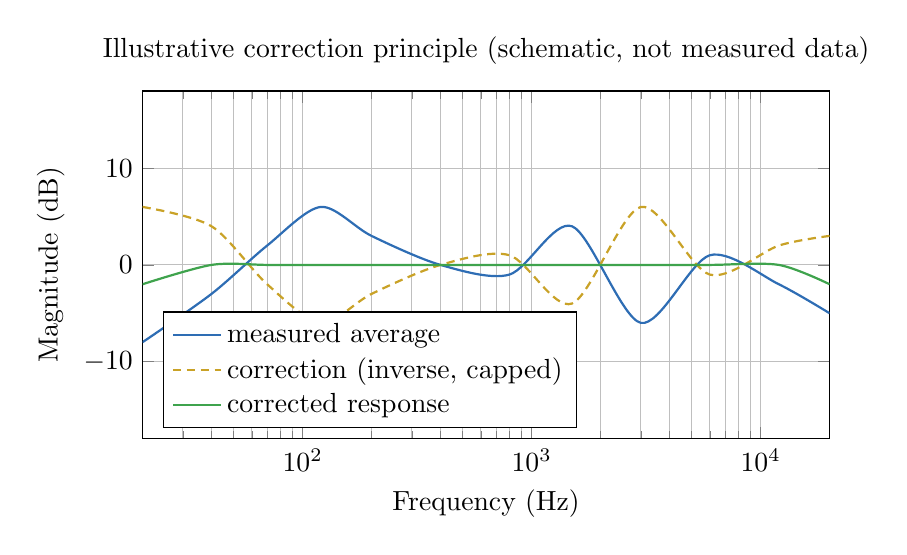
\begin{tikzpicture}
\begin{axis}[
  width=0.85\textwidth, height=6cm,
  xmode=log, xlabel={Frequency (Hz)}, ylabel={Magnitude (dB)},
  xmin=20, xmax=20000, ymin=-18, ymax=18,
  grid=both, legend pos=south west, legend cell align=left,
  title={Illustrative correction principle (schematic, not measured data)}]
% Measured average: a bump + a notch (schematic)
\addplot[thick, smtblue, smooth] coordinates {
  (20,-8)(40,-3)(70,2)(120,6)(200,3)(400,0)(800,-1)(1500,4)
  (3000,-6)(6000,1)(12000,-2)(20000,-5)};
\addlegendentry{measured average}
% Correction: inverse, with LF slope + capped boost
\addplot[thick, smtgold, smooth, densely dashed] coordinates {
  (20,6)(40,4)(70,-2)(120,-6)(200,-3)(400,0)(800,1)(1500,-4)
  (3000,6)(6000,-1)(12000,2)(20000,3)};
\addlegendentry{correction (inverse, capped)}
% Corrected = roughly flat
\addplot[thick, smtgreen, smooth] coordinates {
  (20,-2)(40,0)(70,0)(120,0)(200,0)(400,0)(800,0)(1500,0)
  (3000,0)(6000,0)(12000,0)(20000,-2)};
\addlegendentry{corrected response}
\end{axis}
\end{tikzpicture}
\caption{Schematic of the correction principle: the correction (gold, dashed)
is the regularised inverse of the smoothed measured average (blue); applying
it yields an approximately flat corrected response (green). The boost ceiling
prevents the correction from fully inverting deep notches; the low-frequency
slope rolls the correction off below the target corner. \emph{This plot is
illustrative, not real measurement data.}}
\label{fig:correction}
\end{figure}

\section{Subwoofer phase alignment}
Where a main and a subwoofer overlap around a crossover, their outputs add as
\emph{complex} pressures: a flat summed response requires the two to be in
phase through the crossover region, otherwise the overlap shows a dip (or, if
anti-phase, a deep cancellation)~\cite{Linkwitz1976}. SuperMoTo can steer the
corrected main's phase onto the subwoofer's so the pair sums coherently,
without touching either magnitude.

\subsection{Preserving the relative main/sub timing}
A second measurement set (the subwoofer) is loaded, taken at the \emph{same}
positions as the main and paired by load order. The crucial step is that each
sub measurement is \textbf{delay-anchored on the corresponding main
measurement's delay} rather than having its own delay estimated and removed.
If each file were independently zeroed, the physically meaningful main-vs-sub
arrival-time difference at each position would be discarded; anchoring keeps
it, so the averaged sub response $\bar S(f)$ retains its true phase relative to
$\bar H$.

\subsection{The all-pass alignment term}
From the (unit-magnitude) phase of the sub, $\hat s = \bar S_s/|\bar S_s|$, an
\textbf{all-pass} factor is built and blended towards ``no change'' above the
crossover,
\begin{equation}
  A(f) = \frac{(1-w_x) + w_x\,\hat s(f)}{\bigl|(1-w_x) + w_x\,\hat s(f)\bigr|},
  \qquad C \longmapsto C\cdot A(f),
\end{equation}
where the alignment weight $w_x(f)$ is \textbf{1 at and below the crossover}
and is released to 0 over one octave above it (raised cosine), so the main
keeps its own flat-phase correction in its passband and only inherits the
sub's phase where the two actually overlap. The renormalisation makes $A$
strictly phase-only — \textbf{the main's magnitude correction is unchanged}.
Blending the \emph{phasors} (rather than scaling an unwrapped phase angle)
keeps the rotation on the short arc between $1$ and $\hat s$, so $A$ applies
only the minimal phase shift and never unwinds the sub's large accumulated
low-frequency phase. \textbf{Invert} negates $\bar S$ to flip the sub polarity
if it is wired (or behaves) out of phase. The relative timing comes from the
measurements; physically time-align the drivers with the per-output
\textbf{delays} in the matrix.

\subsection{The complete correction filter}\label{sec:fullfilter}
Collecting the stages of Sections~\ref{sec:correction}--\ref{sec:fullfilter},
the correction applied at each frequency bin is the single complex expression
\begin{equation}
  \boxed{\;
  C(f) = \bigl(1-w(f)\bigr)
       + w(f)\,A(f)\,
         \mathcal{P}_{\lambda}\!\Bigl[\,
           H_{\mathrm{hp}}(f)\;\mathcal{B}\!\bigl[\,1/h(f)\,\bigr]
         \Bigr]\; }
  \label{eq:fullfilter}
\end{equation}
evaluated on the Welch bin grid ($f_k = k\,f_s/W$). It is this spectrum $C(f)$
— not an analytic filter — that Section~\ref{sec:render} resamples and inverse-
transforms into the exported FIR. Reading~\eqref{eq:fullfilter} from the inside
out, the operators are exactly the design steps above:
\begin{align}
  h(f) &= \frac{\bar H_s(f)}{g_{\mathrm{ref}}}
        && \text{normalised smoothed average (Section~\ref{sec:correction}),}\\[2pt]
  \tfrac{1}{h(f)} &= \frac{\overline{h(f)}}{|h(f)|^{2}}
        && \text{exact complex inverse, eq.~\eqref{eq:inverse},}\\[2pt]
  \mathcal{B}[z] &= z\,10^{\,\bigl(\ell(z_{\mathrm{dB}})-z_{\mathrm{dB}}\bigr)/20},\quad
        z_{\mathrm{dB}}=20\log_{10}|z|
        && \text{soft-knee boost limit (phase kept),}\\[2pt]
  \ell(g) &= \begin{cases}
               g, & g \le L-\kappa,\\
               (L-\kappa) + \kappa\tanh\!\dfrac{g-(L-\kappa)}{\kappa}, & g > L-\kappa,
             \end{cases}
        && \kappa=\min(6,L),\ L=\text{max boost (dB)},\\[2pt]
  H_{\mathrm{hp}}(f) &= \frac{(j\omega)^2}{(j\omega)^2+\sqrt{2}\,(j\omega)+1},\quad
        \omega=\frac{f}{f_c}
        && \text{LF slope, } f_c=\SI{30}{\hertz},\\[2pt]
  \mathcal{P}_{\lambda}[z] &= |z|^{\lambda}\,e^{\,j\lambda\arg z}
        && \text{correction level } \lambda\in[0,1],\\[2pt]
  A(f) &= \frac{(1-w_x)+w_x\,\hat s(f)}{\bigl|(1-w_x)+w_x\,\hat s(f)\bigr|}
        && \text{sub phase alignment } (A\equiv 1 \text{ if no sub}),\\[2pt]
  w(f) &\in [0,1]
        && \text{analysis-band weight (raised-cosine skirts).}
\end{align}
Two boundary cases complete the definition: where $|h(f)|$ is negligible the
inverse is replaced by the boost ceiling (rather than diverging), and cuts
($z_{\mathrm{dB}}\le 0$) pass $\mathcal{B}$ unchanged since $L-\kappa\ge 0$ — only
\emph{boosts} are limited. Setting $\lambda=1$, no subwoofer ($A\equiv1$) and a
fully open analysis band ($w\equiv1$) reduces~\eqref{eq:fullfilter} to the
boost-limited, LF-sloped exact inverse $H_{\mathrm{hp}}\,\mathcal{B}[1/h]$.

\section{Rendering the FIR filter}\label{sec:render}
Both exports turn a complex spectrum into a finite impulse response on the
FIR's frequency grid ($N=\text{nextPow2}(\text{firLength})$ bins). The
correction can be rendered in two ways, selected by the \textbf{Phase} control:
\textbf{linear} (mixed-phase) or \textbf{minimum}. The measured-IR export is
always linear-phase.

\subsection{Linear- / mixed-phase rendering}
The resampled spectrum is given a \textbf{half-length linear phase shift} —
multiplying bin $k$ by $e^{-j\pi k}=(-1)^k$ — before the inverse FFT. Because
the correction is a \emph{mixed-phase} filter (it deliberately carries phase
and all-pass content, including the subwoofer alignment, so it is not causal on
its own), centring its energy at sample $N/2$ is what makes it realisable as an
ordinary FIR. A \textbf{Tukey window} (10\,\% taper) centred on $N/2$ then
cleans up the edges. FIR design by frequency sampling and windowing is
standard~\cite{OppenheimSchafer}.

The cost of centring is a constant latency of $\approx N/2$ samples on that
output. SuperMoTo's per-output convolution uses the WDL zero-latency
(uniformly partitioned) convolution engine~\cite{Gardner1995}, so the filter
adds no \emph{algorithmic} block latency beyond that fixed $N/2$ offset — which
the matrix's inter-output latency compensation (Chapter~\ref{ch:matrix}) then
absorbs automatically so all outputs stay time-aligned.

\subsection{Minimum-phase rendering}\label{sec:minphase}
When low latency matters more than phase accuracy — typically \textbf{monitoring
while tracking} — the correction can instead be rendered as a
\textbf{minimum-phase} filter built from its \emph{magnitude alone}. A
minimum-phase response is the unique causal, stable response whose log-magnitude
and phase form a Hilbert-transform pair, so it is fully determined by
$|C(f)|$~\cite{OppenheimSchafer}. SuperMoTo computes it by the real-cepstrum
method: with $c[n]=\mathcal{F}^{-1}\{\log|C|\}$ the real cepstrum, the
minimum-phase log-spectrum is recovered by keeping its causal part,
\begin{equation}
  \hat c[n] = c[n]\,\ell[n], \qquad
  \ell[n] = \begin{cases}
              1, & n=0,\ n=N/2,\\
              2, & 1\le n < N/2,\\
              0, & N/2 < n \le N-1,
            \end{cases}
\end{equation}
and the impulse response is $\mathcal{F}^{-1}\bigl\{\exp \mathcal{F}\{\hat
c\}\bigr\}$, tapered only at the tail (its energy is front-loaded near
$n=0$)~\cite{OppenheimSchafer}. The magnitude correction is \emph{identical} to
the linear-phase version; what is given up is the excess-phase flattening and,
with a subwoofer, the all-pass alignment of Section~\ref{sec:fullfilter} (a
minimum-phase filter cannot impose an arbitrary phase). In return the filter is
causal and front-loaded, so it adds \textbf{essentially no bulk latency}.

Because the inter-output latency compensation keys off each FIR's measured peak
position (Chapter~\ref{ch:matrix}), it recognises the two renderings
automatically: a linear-phase IR reports $\approx N/2$, a minimum-phase IR
reports $\approx 0$, and no special handling is needed. Note, however, that
compensation aligns every fed output to the \emph{longest} engaged FIR, so the
low-latency benefit is only fully realised when \emph{all} engaged outputs use
minimum-phase (or no) FIRs — a single linear-phase FIR in the active
configuration pulls the rest back up to its $N/2$ delay. The on-screen
correction-phase plot always shows the linear-phase design target; in
minimum-phase mode the exported filter matches the displayed \emph{magnitude}
but carries its minimum-phase companion instead.

\section{Exporting}
\begin{itemize}[nosep]
  \item \textbf{Export IR} — saves the \emph{measured} response itself
        (the delay-aligned complex average), band-limited to the analysis range
        so out-of-band room/mic noise does not leak into the file.
  \item \textbf{Export correction IR} — renders the \emph{correction}
        $C$ (Section~\ref{sec:correction}) to a mono \SI{32}{bit}-float wav of a
        selectable FIR length and \textbf{Phase} type (Section~\ref{sec:render}),
        and can assign it directly to an output of the monitoring part. In
        \emph{linear} phase the energy is centred at half the length, adding
        $\text{firLength}/2$ samples of delay on that output (absorbed
        automatically by the inter-output latency compensation); in
        \emph{minimum} phase it is front-loaded and adds essentially none
        (Section~\ref{sec:minphase}).
\end{itemize}

%==============================================================================
\chapter{Workflows}\label{ch:workflows}
%==============================================================================

\section{A — Stereo monitoring with corrected speakers}
\begin{enumerate}[nosep]
  \item Matrix view (or Config tool $\rightarrow$ Stereo 2.0 $\rightarrow$
        Apply to A): route input 1$\rightarrow$out 1, input 2$\rightarrow$out 2.
  \item Calibration, \textbf{Dry} mode: measure outputs 1 and 2, several mic
        positions around the listening spot.
  \item Analysis: load each speaker's set, design the correction,
        \textbf{Export correction IR} and assign it to the output. Repeat per
        speaker.
  \item Calibration, \textbf{FIR} mode: re-measure to verify the corrected
        response is flat.
\end{enumerate}

\section{B — 2.1 / bass-managed system with an aligned subwoofer}
\begin{enumerate}[nosep]
  \item Config tool $\rightarrow$ Stereo 2.1 (or 5.1 / 7.1) $\rightarrow$ set
        the crossover $\rightarrow$ Apply.
  \item Measure and correct each main (workflow A).
  \item Measure the \textbf{sub} alone (Dry) at the same mic positions as one
        main.
  \item Analysis: load the main set, then \textbf{Load sub measurements}; set
        the crossover (toggle \textbf{Invert} if the sub is wired out of
        polarity) — the corrected-main phase is steered onto the sub's through
        the crossover. Export and assign.
  \item Time-align the drivers physically with the per-output \textbf{delays}
        in the matrix; SuperMoTo then automatically delays the sub output to
        match the mains' FIR latency (gold LED on the sub output). Verify in
        Calibration \textbf{System} mode by measuring the input: the summed
        response should be smooth through the crossover.
\end{enumerate}

\section{C — Verifying the complete system end to end}
Calibration, \textbf{System} mode, select the plugin input your source uses.
The stimulus runs through the engaged configuration exactly as monitored
(routing, crossover, FIRs, latency compensation). Analysis of that capture
shows the real in-room system response.

\section{D — Multiple speaker sets / quick A/B}
Store different rigs or rooms in configurations A--F (e.g.\ A = mains,
B = mains+sub, C = nearfields) and switch from the top bar. Use
\textbf{Exclusive} for A/B, non-exclusive to sum. Collapse
(\textbf{$\blacktriangle$}) to a compact output-strip-only window.

%==============================================================================
\chapter{Building from source}\label{ch:build}
%==============================================================================

SuperMoTo is CMake based and mirrors the MechanOdd project layout. JUCE and
the FxmeJuceTools user module are expected as siblings of the repository:

\begin{verbatim}
../JUCE/                              juce-framework/JUCE checkout
../JUCE/usermodules/FxmeJuceTools/    symlink to FxmeJuceTools/module/FxmeJuceTools
\end{verbatim}

\begin{verbatim}
git submodule update --init --recursive   # FxmeFX + WDL
cmake -B build -DCMAKE_BUILD_TYPE=Release
cmake --build build -j
\end{verbatim}

Produced formats: VST3, AU, Standalone (16 discrete in / 16 discrete out).
Continuous-integration builds for Linux, macOS (universal) and Windows are
provided by the GitHub Actions workflow \texttt{.github/workflows/release.yml},
triggered by pushing a version tag (\texttt{v\textit{X.Y.Z}}).

\section{License}
LGPL-3.0-or-later — \textcopyright{} 2023--2026 Olivier Doaré.

%==============================================================================
\begin{thebibliography}{99}
%==============================================================================

\bibitem{Welch1967}
P.~D. Welch, ``The use of fast Fourier transform for the estimation of power
spectra: A method based on time averaging over short, modified periodograms,''
\textit{IEEE Trans. Audio Electroacoust.}, vol.~15, no.~2, pp.~70--73, 1967.

\bibitem{BendatPiersol}
J.~S. Bendat and A.~G. Piersol, \textit{Random Data: Analysis and Measurement
Procedures}, 4th ed. Hoboken, NJ: Wiley, 2010.

\bibitem{ShinHammond}
K.~Shin and J.~K. Hammond, \textit{Fundamentals of Signal Processing for Sound
and Vibration Engineers}. Chichester: Wiley, 2008. (Frequency-response
estimators $H_1$/$H_2$ and the coherence function.)

\bibitem{OppenheimSchafer}
A.~V. Oppenheim and R.~W. Schafer, \textit{Discrete-Time Signal Processing},
3rd ed. Upper Saddle River, NJ: Prentice Hall, 2010.

\bibitem{Harris1978}
F.~J. Harris, ``On the use of windows for harmonic analysis with the discrete
Fourier transform,'' \textit{Proc. IEEE}, vol.~66, no.~1, pp.~51--83, 1978.

\bibitem{MullerMassarani}
S.~Müller and P.~Massarani, ``Transfer-function measurement with sweeps,''
\textit{J. Audio Eng. Soc.}, vol.~49, no.~6, pp.~443--471, 2001.

\bibitem{Hatziantoniou2000}
P.~D. Hatziantoniou and J.~N. Mourjopoulos, ``Generalized fractional-octave
smoothing of audio and acoustic responses,'' \textit{J. Audio Eng. Soc.},
vol.~48, no.~4, pp.~259--280, 2000.

\bibitem{Mourjopoulos1994}
J.~N. Mourjopoulos, ``Digital equalization of room acoustics,''
\textit{J. Audio Eng. Soc.}, vol.~42, no.~11, pp.~884--900, 1994.

\bibitem{NeelyAllen}
S.~T. Neely and J.~B. Allen, ``Invertibility of a room impulse response,''
\textit{J. Acoust. Soc. Am.}, vol.~66, no.~1, pp.~165--169, 1979.

\bibitem{Kirkeby1999}
O.~Kirkeby and P.~A. Nelson, ``Digital filter design for inversion problems in
sound reproduction,'' \textit{J. Audio Eng. Soc.}, vol.~47, no.~7/8,
pp.~583--595, 1999.

\bibitem{Toole}
F.~E. Toole, \textit{Sound Reproduction: The Acoustics and Psychoacoustics of
Loudspeakers and Rooms}, 3rd ed. New York: Routledge, 2017. (Spatial averaging
and the case against single-point room correction.)

\bibitem{Linkwitz1976}
S.~H. Linkwitz, ``Active crossover networks for noncoincident drivers,''
\textit{J. Audio Eng. Soc.}, vol.~24, no.~1, pp.~2--8, 1976.

\bibitem{Gardner1995}
W.~G. Gardner, ``Efficient convolution without input-output delay,''
\textit{J. Audio Eng. Soc.}, vol.~43, no.~3, pp.~127--136, 1995.

\end{thebibliography}

\end{document}
